\documentclass[zihao=-4]{ctexart}
\usepackage[normalem]{ulem}
\useunder{\uline}{\ul}{}
%********************导言区宏包引入********************
\usepackage{xeCJK}
\usepackage{amssymb}
\usepackage{amsmath}
\usepackage{listings} %代码
\usepackage{graphicx}
\usepackage{multicol} %回车换段
\usepackage{xcolor}
\usepackage{geometry} %页面设置
\usepackage{fontspec}
\usepackage{setspace}
\usepackage{times}
\usepackage{fancyhdr} %页眉页脚
\pagestyle{fancy}
\usepackage{float} %表格位置
\usepackage{titlesec} %设置
\usepackage{titletoc}
\usepackage{ctex}
\usepackage{gbt7714}    %控制参考文献格式为国标
\usepackage{multirow}
\usepackage{booktabs}   %表格相关
\usepackage{setspace}   %设置行距
\usepackage{caption} %caption
\usepackage{subcaption} %子图的caption
\usepackage{changepage} %左右缩进

\graphicspath{ {pictures/} }
\let\algorithm\relax
\let\endalgorithm\relax
\usepackage[ruled,vlined]{algorithm2e}%[ruled,vlined]{
\usepackage{algpseudocode}
\renewcommand{\algorithmicrequire}{\textbf{Input:}} 
\renewcommand{\algorithmicensure}{\textbf{Output:}}
%\renewcommand\thepage{\zihao{-5} ~\arabic{page}~}%页码字号

%定义两个arg
\DeclareMathOperator*{\argmax}{arg\,max}
\DeclareMathOperator*{\argmin}{arg\,min}
\DeclareCaptionLabelSeparator{mysep}{\space\space}  %自定义caption格式
\captionsetup[figure]{font={small}, labelfont=bf, labelsep=mysep, textfont=bf}   %图片caption格式
\captionsetup[table]{font={small}, labelfont=bf, labelsep=mysep, textfont={bf}}   %表格caption格式
\bibliographystyle{gbt7714-numerical} %修改了title斜体内容

%********************导言区宏包引入********************
%********************第三方字体引入********************
%\setCJKmainfont[Path=fonts/,BoldFont=simhei.ttf,ItalicFont=simkai.ttf,SlantedFont=simfang.ttf]{simsun.ttc}
%中文字体涵盖黑体、宋体、楷体、仿宋
\setmainfont[Path=fonts/, 
BoldFont = times-new-roman-bold.ttf,
ItalicFont = times-new-roman-italic.ttf,
BoldItalicFont = times-new-roman-bold-italic.ttf
]{times-new-roman.ttf}
\setmonofont[Path=fonts/]{Courier New.ttf}
\setCJKfamilyfont{hwzs}[Path=fonts/]{STKzhongsong.ttf}%使用STZhogsong华文中宋字体
\newcommand{\zhongsong}{\CJKfamily{hwzs}}
\setCJKfamilyfont{hwxw}[Path=fonts/]{STKxinwei.ttf} % XSP 2023/3/3:
\newcommand{\xinwei}{\CJKfamily{hwxw}}              %  使用STZxinwei华文新魏字体.

%********************第三方字体引入********************

%********************代码段设置********************
% by yjw
% \texttt 用于行内代码,等宽字体,不知道让不让用
\usepackage{listings} % 用于代码排版
\usepackage{xcolor} % 用于代码高亮
% 定义代码块样式
\lstdefinestyle{codeblock}{
    backgroundcolor=\color{white},    % 背景颜色
    basicstyle=\ttfamily\small\fontsize{9pt}{8pt}\selectfont, % 设置字体大小和行间距
    breakatwhitespace=false,          % 是否只在空白处自动断行
    breaklines=true,                  % 自动断行
    captionpos=b,                     % 标题位置
    commentstyle=\color{gray},        % 注释风格
    frame=single,                     % 单框
    keepspaces=true,                  % 保持空格
    keywordstyle=\color{blue},        % 关键字风格
    numbers=left,                     % 行号位置
    numbersep=8pt,                    % 行号与代码的距离
    numberstyle=\tiny\color{gray},    % 行号样式
    rulecolor=\color{black},          % 框架颜色
    showspaces=false,                 % 不显示空格
    showstringspaces=false,           % 字符串中不显示空格
    showtabs=false,                   % 不显示制表符
    stepnumber=1,                     % 步长
    stringstyle=\color{orange},       % 字符串风格
    tabsize=2,                        % 制表符占用空格数
    xleftmargin=\parindent,           % 左边距
    framexleftmargin=12pt,            % 框架左边距,增加些许间距以包含行号
}
\captionsetup[lstlisting]{font={small}, labelfont=bf, labelsep=mysep, textfont=bf}
\renewcommand{\lstlistingname}{伪代码}
\lstset{style=codeblock}
%********************代码段设置********************

%********************中文字号设置********************
%\newcommand{\chuhao}{\fontsize{42pt}{\baselineskip}\selectfont}
\newcommand{\chuhao}{\fontsize{42pt}{0}}
\newcommand{\xiaochu}{\fontsize{36pt}{0}}
\newcommand{\yihao}{\fontsize{28pt}{0}}
\newcommand{\erhao}{\fontsize{21pt}{0}}
\newcommand{\xiaoer}{\fontsize{18pt}{0}}
\newcommand{\sanhao}{\fontsize{16pt}{0}}
\newcommand{\sihao}{\fontsize{14pt}{0}}
\newcommand{\xiaosi}{\fontsize{12pt}{0}}
\newcommand{\wuhao}{\fontsize{10.5pt}{0}}
\newcommand{\xiaowu}{\fontsize{9pt}{0}}
\newcommand{\liuhao}{\fontsize{8pt}{0}}
\newcommand{\qihao}{\fontsize{5.25pt}{0}}
%********************中文字号设置********************


%********************页边距设置********************
\geometry{left=3cm,right=2cm,top=2.5cm,bottom=2.5cm}
\geometry{a4paper} % xsp 2023/3/7: 调整纸张大小为A4
%********************页边距设置********************

%********************段间距设置********************
\newcommand{\setParDis}{\setlength {\parskip} {0pt} }
%请在每部分使用这个
%********************段间距设置********************

%********************子文件导入区域****************
% 用于仅编译部分导入文件
% \includeonly{subtexs/ros_background, }

\begin{document}
%********************页眉页脚设置********************
\lhead{}%设置左页眉为空
\rhead{}%设置左页眉为空
\setlength{\headwidth}{\textwidth}% 2023/3/3 XSP: 页眉长度适应文本
%********************页眉页脚设置********************


%********************标题格式设置********************

%\setcounter{secnumdepth}{0}%该命令取消了章标题前数字label

\CTEXsetup[name={,、},number={\chinese{section}}]{section}
\CTEXsetup[name={(,)},number={\chinese{subsection}}]{subsection}
\CTEXsetup[name={,.},number={\arabic{subsubsection}}]{subsubsection}% 不加会导致目录格式错误
% 设置subsubsection等格式
% \titleformat{\section}[block]{\sanhao\bfseries\centering}{\chinese{section}、}{0pt}{}[]
% \titleformat{\subsection}[block]{\sihao\bfseries}{(\chinese{subsection})}{0pt}{}[]
% \titleformat{\subsubsection}[block]{\xiaosi\bfseries}{\arabic{subsubsection}、}{0pt}{}[]
\titleformat{\section}[block]{\sanhao\heiti\centering}{\chinese{section}、}{0pt}{}[]    % XSP 2023/3/3:
\titleformat{\subsection}[block]{\sihao\heiti}{(\chinese{subsection})}{0pt}{}[]       %   将正文标题字体由加粗
\titleformat{\subsubsection}[block]{\xiaosi\heiti}{\arabic{subsubsection}.}{0pt}{}[]   % 修改为黑体。
\titlespacing{\section}{0pt}{25pt}{12pt}
\titlespacing{\subsection}{0pt}{7pt}{7pt}
\titlespacing{\subsubsection}{0pt}{5pt}{4pt}

\titlecontents{section}[1.6em]{\addvspace{2pt}\filright}
{\contentspush{\thecontentslabel\hspace{0.8em}}}
{}{\titlerule*[8pt]{.}\contentspage}

\titlecontents{subsection}[3.2em]{\addvspace{2pt}\filright}
{\contentspush{\thecontentslabel\hspace{0.8em}}}
{}{\titlerule*[8pt]{.}\contentspage}

\titlecontents{subsubsection}[6.4em]{\addvspace{2pt}\filright}
{\contentspush{\thecontentslabel\hspace{0.8em}}}
{}{\titlerule*[8pt]{.}\contentspage}
%********************标题格式设置********************

%\setcounter{section}{-3}  %标题计数器
%\stepcounter{section}

%*******************行间距段前段后*******************
\linespread{1.8}
%行间距为实际行间距乘以1.2,如此处实际为1.5倍行距
\setlength{\parskip}{0.5\baselineskip}
%*******************行间距段前段后*******************



%********************封面部分********************
%
%     论文题目:应准确、鲜明、简洁,能概括整个论文中最主要和最重要的内容。
% 题目不超过20个中文字,若语意未尽,可用副标题补充说明。副标题应处于从属
% 地位,一般可在题目的下一行用破折号“——”引出。论文题目应避免使用不常用缩
% 略词、首字母缩写字、字符、代号和公式等。
%
\def\Fengru{第三十四届“冯如杯”竞赛主赛道}
\leftline{\includegraphics[scale=1]{pictures/xiaohui.png}} % XSP 2023/3/3: 取消校徽段首缩进
%格式控制部分
% \par \  
% \par \
% \par \
\vspace{32pt}
\begin{center}
\includegraphics[height=2.25cm, width=12.78cm, scale=1]{pictures/xiaoming.png}
\end{center}
%格式控制部分
\vspace{12pt}

\begin{spacing}{3}
    % \erhao
    \begin{center}
      {
        \fontsize{22pt}{3}\selectfont
        \zhongsong{针对机器人操作系统的自动测试框架} 
      } 
        % \zhongsong{“冯如杯”竞赛主赛道项目是什么}
    \end{center}
    \rightline{\xinwei\sanhao{——基于模糊测试技术}} % XSP 2023/3/3: 副标题二号华文新魏居右
\end{spacing}
%格式控制部分
\par \ 
\par \
\par \ 
\par \


%格式控制部分
\par \ 
\begin{center}
\sanhao
\centerline{\heiti{}}%封面年月去掉
\end{center}

\pagenumbering{gobble} %封面无页码
%\thispagestyle{empty}


\renewcommand{\headrulewidth}{0pt}%没有页眉装饰线
\clearpage
\pagenumbering{roman} %摘要目录页小写罗马

\xiaosi
\section*{摘要}
\begin{spacing}{1.5}
  \setParDis %设置段间距为 0
% 500z字? 目的, 意义, 研究方法, 成果, 结论
商用机器人、自动驾驶等领域的快速发展,带动了相关软件工具的进步。其中,机器人操作
系统(ROS2),以其开源、跨平台、高效的软件框架及丰富的工具库而深受开发者喜爱,在
学界、商业应用中得到广泛应用。与此同时,机器人操作系统也存在开源软件共有的安全漏
洞多、不稳定等问题,制约着其进一步发展,也威胁着相关应用的安全。

机器人操作系统相关程序亟需一种高效的测试方法,面对这一场景,我们选择将自动模糊测
试技术(Fuzzing)引入对机器人操作系统的测试。通过随机变异测试输入,并加入反馈引
导,模糊测试不仅提高了测试的自动化程度,还能有效地探索软件异常路径,揭露隐蔽漏
洞,显著改善了传统软件测试方法的繁琐性和低效性。

为了提高测试效率,我们的模糊测试对机器人系统进行针对性优化。针对通信网络环境的不
稳定性,本框架选择将机器人收到的通信消息等多维度输入进行随机化变异;针对机器人多
进程多线程的软件特点,本框架通过程序插桩延迟来提高数据竞争概率;针对机器人程序弱
状态特点,本框架通过流量分析等黑盒手段,来辅助推测程序内部状态。

本作品设计的测试框架短期内共发掘28个ROS2相关软件的内存漏洞、并发漏洞,其中11个得
到开发者确认修复,其中有4个重要漏洞被美国通用漏洞披露(CVE)收录,7个通过中国国
家漏洞库(CNVD)二级审核,正在等待三级审核。

综上,本作品——针对机器人系统的模糊测试框架在软件测试中有较高实践价值,已为开源社
区贡献多次漏洞修复,并可高效地移植用于测试其他机器人程序。


\end{spacing}
    
\textbf{关键词:}自动模糊测试技术,机器人操作系统,并发漏洞检测,内存安全漏洞检测

\newpage
\section*{\textbf{Abstract}} % XSP 2023/3/8: Abstract 加粗
\begin{spacing}{1.5}
\begin{adjustwidth}{0.42cm}{0.42cm}
\setParDis %设置段间距为 0

\noindent\hspace{\parindent}The swift advancement in commercial robotics and
autonomous driving has spurred the development of associated software tools,
notably the Robot Operating System (ROS2). Celebrated for its open-source,
cross-platform capabilities, and extensive toolkit, ROS2 has garnered widespread
adoption across academia and industry. However, its growth is hampered by common
open-source software issues like security vulnerabilities and instability,
posing risks to application safety.

Addressing the need for efficient testing in \textbf{ROS2-related programs}, we
introduced automatic \textbf{fuzz} testing to enhance software reliability. By
employing randomized mutations of test inputs and feedback guidance, fuzz
testing significantly elevates automation and efficacy in exploiting
vulnerabilities, outpacing traditional testing in identifing uncovering software
exception.

Our framework, tailored for robotic systems, addresses communication network
instability by randomizing inputs like received communication messages. It
targets software's multi-process and multi-threaded nature by increasing data
race probabilities via program instrumentation delays. Additionally, to navigate
the challenges posed by robots' weak states, our framework utilizes black-box
methods, such as traffic analysis, to infer internal states. The approach led to
\textbf{the discovery of 28 ROS2 software vulnerabilities, with 11 confirmed and
fixed by developers, including 4 recognized by the US's CVE and 7 awaiting final
review by China's CNVD.}

This work demonstrates the high practical value of our fuzz testing framework
for robotic systems, contributing significantly to the open-source community and
efficiently adaptable for testing various robot programs.

\textbf{Keywords: Fuzz, ROS2, Concurrent Vulnerability, Memory Vulnerability}
\end{adjustwidth}
\end{spacing}
%********************摘要部分********************

%********************目录部分********************
\clearpage
\tableofcontents
\clearpage
%********************目录部分********************

\renewcommand{\headrulewidth}{0.4pt} %恢复页眉装饰线

%********************正文页眉部分********************
%\lhead{} 
\chead{\xiaowu 北京航空航天大学\Fengru 参赛作品} %设置居中页眉
%********************正文页眉部分********************

\pagenumbering{arabic} %正文页码从1开始,用阿拉伯数字
\setcounter{page}{1} 

%******************* 一 作品概述************************
\section{作品概述}
\setParDis %设置段间距为 0
\begin{spacing}{1.5} % 行距1.5


\subsection{背景介绍} %@author: lhy
% \subsection{背景介绍}
%@author: lhy
\subsubsection{ROS系统重要性}
人类生活与机器人密不可分。传统上,机器人在农业和制造业中被广泛用于任务自动化。最
近的发展让机器人更加贴近每个人的日常生活。例如,亚马逊和谷歌正在部署无人配送系统
,使用无人驾驶飞行器,机器人吸尘器的市场规模年增长率达到23\%,以及在
2012年到2018年间,使用机器人进行手术的比例从2\%增加到15\%,显示出机器人产业
为适应人类需求而快速增长的态势。同时,现代机器人,如自动驾驶车辆,正在变得更加复
杂,要求集成复杂的子系统,例如感知、感觉、规划和执行。

为了应对开发复杂机器人系统的更高需求,机器人操作系统(ROS)$^{[15]}$正在获得越来越多的
关注。ROS是一个开源的中间件套件,用于机器人开发,它具有分布式机器人进程的消息传
递机制、硬件抽象、广泛的开发工具(例如,模拟器)和机器人库(例如,路径规划算
法)。使用ROS,开发者可以加速开发过程,无需重新发明轮子,而是可以专注于他们机器
人的核心功能。凭借其多语言和多平台支持的理念,ROS正在成为机器人编程中的实际标
准;它已被广泛采用于工业、军事、研究机构以及个人,预计到2024年将为
55\%的商业机器人提供动力。近些年ROS系统相关论文数量与Wiki用户数量如图1所示:

\begin{figure}[H]
  \centering
  \includegraphics[width=11cm]{ros_papers.png}
  \caption{ROS系统相关论文数量与Wiki用户数量}
\end{figure}

机器人操作系统(ROS)是一个开源平台,它为用C++和Python等不同语言实现机器人软件提
供了许多实用的工具和库。超过740家商业公司正在使用ROS$^{[16]}$来开发数百种实际应用的机
器人$^{[17]}$,这表明了其在机器人开发中的流行度。然而,开发可靠的ROS程序具有挑战性,因
为机器人可以在复杂的物理环境中工作,并可能遇到各种异常情况(如无效的配置参数和异
常的传感器信息)。如果ROS程序不够可靠,它们的错误可能在与人类和其他机器人交互时
导致危险事故。

ROS本身的缺陷或者开发者在应用中常用的ROS使用方式可能会影响依赖于ROS的广泛机器人
系统,并对许多用户的安全和保障造成严重破坏。例如,ROS版本1没有认证的概念,允许网
络上的任何实体完全访问任何机器人系统,窃听内部消息,甚至在知道IP地址和端口的情况
下劫持执行。实际上,在互联网上扫描默认的ROS端口两个月后,发现部署在28个国家的超
过100个ROS系统,这些系统完全暴露于此类攻击之下。ROS的最新版本(即ROS 2)在设计和
实现时考虑了这些问题,并邀请了更广泛的公众对安全性进行审查。不幸的是,现有的工作
和解决方案要么专注于关于认证和授权方法的网络安全方面,要么专注于回归测试,使得
ROS社区在寻找影响机器人系统的健壮性和正确性的未知错误方面缺乏一种系统的测试方
法。

\subsubsection{自动驾驶兴起与ROS}
自动驾驶技术的兴起标志着交通运输领域的一次重大革命,其不仅预示着交通安全、效率和
环境影响的根本改进,而且还预示着个人出行和货物运输方式的深刻变革,而这一过程在很
大程度上得益于机器人操作系统(Robot Operating System,ROS)的发展和应用。近年
来,由于计算能力的显著提升、大数据技术的发展、人工智能算法的进步以及传感器技术的
优化,自动驾驶汽车从理论研究和小规模试验逐步走向了公路测试和商业化应用的初步阶
段。

根据国际汽车工程师学会(SAE)的定义$^{[15]}$,自动驾驶分为六个级别,从0级(无自动化)到5
级(完全自动化)。目前,多数公开测试和部分商业化应用的自动驾驶汽车处于3级(有条
件自动化)到4级(高度自动化)。尽管完全自动化(5级)的汽车尚未广泛部署,但多个技
术开发者和制造商已经在进行相关的研发工作,并在不同国家和地区开展了路试。

随着自动驾驶技术的进步,对处理大量传感器数据、实现复杂决策逻辑和执行精确控制的需
求不断增加,ROS的可扩展性和灵活性在此过程中显示出其不可或缺的价值。例如,ROS的消
息传递系统支持多种编程语言,允许异构系统高效集成。此外,其庞大的开源社区贡献了大
量的软件包,覆盖从3D视觉到路径规划等各种功能,极大地丰富了自动驾驶汽车的研发资源
库。

经济学人智库的一份报告预测,到2035年,全球自动驾驶汽车的数量将达到近7500万
辆。而麦肯锡公司的一项研究则估计$^{[16]}$,自动驾驶技术的全面部署将使交通事故造成的死
亡人数减少90\%,同时还将大幅度提升道路运输效率和减少碳排放。图2展示了PRECEDENCE
RESEARCH机构预测的未来自动驾驶市场规模:

\begin{figure}[H]
  \centering
  \includegraphics[width=0.8\textwidth]{market_size.png}
  \caption{自动驾驶市场规模}
  \label{fig:my_label}
\end{figure}

尽管自动驾驶技术的前景被广泛看好,但其商业化应用和普及还面临多重挑战,包括技术完
善度、法律法规、道德伦理、消费者接受度以及基础设施配套等。例如,自动驾驶汽车在复
杂的城市交通环境中的表现,以及在极端天气条件下的可靠性,仍然是技术研发中的重要挑
战。

未来,随着相关技术的进一步成熟和相关政策的完善,自动驾驶汽车有望在更广泛的领域得
到应用,从而实现对交通系统的根本性改造和优化。这将不仅影响交通运输本身,还将对城
市规划、能源消费、环境保护以及人们的生活方式产生深远影响。

\subsubsection{自动驾驶产生漏洞的危害}
尽管自动驾驶汽车(AVs)承诺通过减少人为错误来增加道路安全,它们固有的技术漏洞却
可能导致严重的安全后果。据国家公路交通安全管理局(NHTSA)估计,94\%的严重交通事
故是由人为因素引起的,而自动驾驶技术的开发者们宣称,通过消除这一因素,可以极大地
提高道路安全性$^{[18]}$。然而,这种安全性的提升假设基于自动驾驶系统能够无缺陷地执行其
预定任务,这在实践中往往难以实现。

自动驾驶汽车的技术漏洞主要分为两类:软件漏洞和硬件故障。软件漏洞包括但不限于算法
错误、安全漏洞以及对异常情况的处理不足。硬件故障可能涉及传感器故障、执行机构的故
障或其他关键组件的损坏。这些技术漏洞不仅可能导致单一车辆的操作失败,还可能对整个
交通系统产生连锁反应,特别是在高度自动化和互联的交通环境中。

例如,2018年3月,在美国亚利桑那州发生了一起致命的自动驾驶汽车事故,一名行人在穿
越街道时被一辆自动模式下的Uber汽车撞击,导致死亡。初步调查显示,该事故部分原因是
系统无法正确识别并响应行人$^{[19]}$。这一事件凸显了即使在自动驾驶技术取得显著进步的情
况下,技术漏洞仍然可能导致灾难性后果。

此外,安全研究人员已经证明,自动驾驶汽车系统的安全漏洞可以被黑客利用,进而控制车
辆的行驶方向或速度,造成严重安全威胁$^{[20]}$。例如,通过篡改车辆的环境感知系统接收到
的数据,攻击者可以使汽车忽略停车标志或其他关键交通信号,导致交通事故。

综上所述,尽管自动驾驶技术和机器人技术被寄予厚望,但频繁出现的技术漏洞和安全威
胁,表明相关技术的安全可靠性还需要进一步提高。因此,对相关程序和基础ROS2系统的进
一步安全测试、漏洞排除仍然任重道远,亟需新技术来高效、无痛地排除漏洞威胁,降低技
术进步的血泪代价。



\subsection{研究现状}
% 这里衔接一下为什么我们想将模糊测试应用到ROS上

\subsubsection{ROS常见测试方案}
%@author: yjw
%TODO: 审核,文献,表格格式
近期有几种$^{[2, 6, 7, 8, 9, 10]}$应用于ROS2程序的新型测试方法,它们不同于由开发者手动构造测试样例的单元测试,而尝试自动生成ROS程序输入,并借助清洁工具(Sanitizer)自动监控程序内存或语义错误。它们大幅提高了针对机器人系统的测试效率,表\ref{tab:fuzzers}将这些方法进行了比较(包括本作品),可以看出这些方法在测试ROS程序时仍存在三个主要限制:

\textbf{限制一:}测试用例生成效率低。大部分测试方法从单一维度(即用户命令或传感器信息)生成输入,并且生成的测试样例随机性过强,无法识别出可能高效探索程序边界的变异维度,导致许多生成的输入无助于增加测试覆盖率。

\textbf{限制二:}程序反馈效果不佳。SMACH-Fuzz和ASTAA随机生成输入,而没有反馈和指导;Ros2-fuzz和ROZZ参考AFL工具$^{[11]}$使用代码覆盖率作为程序反馈,但代码覆盖率对多进程运行情况不敏感,且忽略了不同执行路径;Phys-Fuzz使用场景危险程度评分来指导进一步生成场景,对于检测ROS2自动导航程序的避障能力效果较好,但也仅限制在了此场景下;RoboFuzz使用语义反馈来量化机器人执行上下文的正确性,但是这种特殊语义的设计编写需要很强专业知识。

\textbf{限制三:}自动化水平低。大部分方法都需要大量领域特定知识和手动努力来配置输入生成规则(ASTAA和RoboFuzz),编写有关机器人行为的规格(SMACH-Fuzz和RoboFuzz),检查执行日志(SMACH-Fuzz和Phy-Fuzz)等,这导致测试效率和便捷程度对比传统单元测试并没有很大提高。

\begin{table}[H]
\small
\centering
\caption{最新针对ROS系统的测试技术对比}
\begin{tabular}{lccccc}
\hline
\textbf{技术名} & \textbf{输入维度}  & \textbf{反馈}& \textbf{自动化程度} & \textbf{漏洞类型} \\ \hline
SMACH-Fuzz $^{[6]}$ & 单一 & 无 & 差 & 行为错误 \\ 
Phys-Fuzz $^{[7]}$ & 单一  & 环境危险程度  & 差& 碰撞损坏 \\ 
Ros2-fuzz $^{[10]}$ & 单一  & 代码覆盖率   & 较好 & 内存漏洞 \\ 
ASTAA $^{[8]}$ & 单一 & 无 & 差 & 行为错误 \\ 
RoboFuzz $^{[9]}$ & 单一  & 语义反馈 & 较差 & 行为错误 \\ 
ROZZ $^{[2]}$ & 多维度 & 代码覆盖率 & 较好 & 内存漏洞 \\ 
本作品 & 多维度  & 代码覆盖率+流量分析 & 较好& 内存与并发漏洞 \\ \hline
\end{tabular}
\label{tab:fuzzers}
\end{table}


\subsubsection{模糊测试及其应用}
%@author: jfb
模糊测试是近年来最受欢迎的软件测试技术之一,通过向系统输入异常、随机或无效的数据
来暴露软件中的缺陷、漏洞和崩溃。模糊测试在不需要了解应用程序内部逻辑的情况下,检
测软件如何处理意外或错误的输入,非常适合寻找安全漏洞,如缓冲区溢出、执行流程控制
错误、内存泄露等。同时,利用模糊测试发现了许多高影响力的安全漏洞(如
Heartbleed、Shellshock等),进一步证明了其有效性和重要性。

尽管模糊测试在软件安全领域得到了广泛应用,但在ROS环境中的应用相对较少。随着人工
智能技术的发展和ROS在人工智能如无人驾驶等研究及应用中的重要性增加,对于ROS环境的模
糊测试方法的需求和研究也在逐渐增长。开发专门针对ROS系统特点的模糊测试工具和技
术,可以有效提高机器人软件的可靠性和安全性。

\subsection{作品概述}
%@author: yjw
% author: yjw
本作品给出针对ROS2系统的自动模糊测试程序,其核心框架如图\ref{pic:off}所示,旨在提高对ROS2系统相关的自动驾驶项目、机器人项目的漏洞测试的便捷性和高效性,为开发者提供一个有效测试工具。开发者首先将源码搭配本作品的编译器工具编译为可执行程序,此过程中本作品将自动使用LLVM架构对源码进行插桩修改,并链接相应清洁程序(如Address Sanitizer等第三方监控工具);接着,本作品核心模糊测试驱动器会启动特殊ROS2执行环境执行开发者的ROS2程序,并将开发者提供的初始测试样例进行变异修改,生成一个测试用例输入进程序;本作品的监控器(Node Monitor)会对被测程序的代码覆盖率、程序异常、通信流量、服务状态等信息进行收集分析;分析结果被作为该测试用例种群适应度输入到遗传算法中,遗传算法会对种群(测试用例池)进行进化和淘汰,选择出更有可能触发程序边界的测试用例,并指导对测试用例种群进行进一步变异。

\begin{figure}[H]
    \centering
    \includegraphics[width=14cm]{our_fuzz_framework.png}
    \caption{本项目实现的Fuzz框架}
    \label{pic:off}
\end{figure}

通过上述步骤,本作品会不断生成被测ROS2节点程序的高质量测试用例,覆盖更多节点程序的内部状态分支,以更高效率探索程序潜在漏洞。本作品的创新之处主要有几点:针对ROS2系统程序特点,不局限于传统测试输入,探索多维度的程序输入;以更高效的办法对ROS2节点程序进行监控,综合白盒插桩检测与黑盒流量分析等技术;支持检测多种漏洞类型,如内存安全漏洞与并发漏洞等。

% 终极版本是一个魔改的ROS环境,包括魔改DDS,魔改RCLCPP链接库,Tracing守护进程(流量分析),一个Node可以不运行在其项目整个系统中,如测试Navigation2中的Nav2 AMCL可以不运行整个系统,魔改ROS环境会自动接管其所有接口,进行输入变异


%*********************** 二 作品设计与实现***************
\section{作品设计与实现}
\setParDis %设置段间距为 0

\subsection{技术背景与预备知识} %@author: wkt, yjw, jfb
\begin{enumerate}
	\item 释放后使用(UAF):
	
	释放后使用问题发生在程序试图使用已释放的内存时。通常,内存释放后,操作系统会将该内存标记为可重新使用,但并不会立即清空其内容。如果程序在内存释放后继续访问该内存,就可能导致安全漏洞。该漏洞的介绍如图1所示。
	\begin{figure}[htbp]
		\centering
		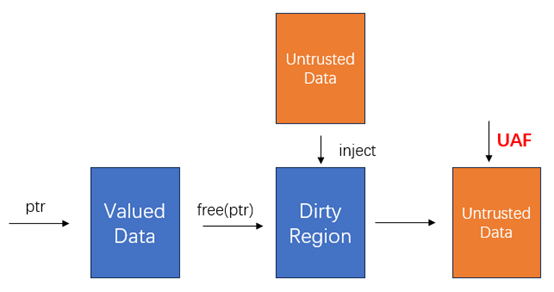
\includegraphics[width=0.5\textwidth]{pictures/UAF.png}
		\caption{释放后使用漏洞图示}
		\label{fig:UAF}
	\end{figure}
	攻击者可能利用释放后使用漏洞来执行未经授权的代码,例如通过释放内存但保留对其的引用,然后在后续代码中使用该引用,从而导致恶意代码执行。同时可能导致程序崩溃或不稳定,因为操作已释放的内存区域可能导致未定义的行为。
	
	Heartbleed漏洞是一个广为人知的释放后使用漏洞的例子。该漏洞影响了OpenSSL库中的Heartbeat扩展,攻击者可以发送恶意的Heartbeat请求,从而导致服务器上的内存泄漏和可能的敏感信息泄露。
	
	\item 异常(Exception):
	
	异常是一种用于处理错误或不正常情况的机制。在程序执行期间,如果发生异常,通常会中断当前执行流程,并转移到异常处理代码。如果程序未正确处理异常,可能会导致安全漏洞。
	
	异常可能导致程序跳转到未经测试的代码路径,使得程序执行流程不可预测,从而导致意外行为或安全漏洞。同时,异常通常包含程序执行的上下文信息,攻击者可能利用这些信息来进一步渗透系统,进而导致信息泄露。
	
	在2014年的``Shellshock''漏洞中,攻击者利用了Unix/Linux系统中的一个bash
	shell的异常处理漏洞。通过在HTTP请求的User-Agent头中注入恶意代码,攻击者能够利用bash的异常处理漏洞来执行任意命令,从而导致系统被入侵。
	
	\item 缓冲区溢出(Buffer overflow):
	
	缓冲区溢出发生在程序试图向一个缓冲区写入超过其分配大小的数据时。这导致数据溢出到相邻的内存区域,覆盖了那些数据或程序代码。通常,这种溢出可以修改程序的执行流程,因为溢出数据可能包含特定的指令地址,攻击者可以利用这一点来控制程序的行为。该漏洞的介绍如图2所示。
	
	\begin{figure}[htbp]
		\centering
		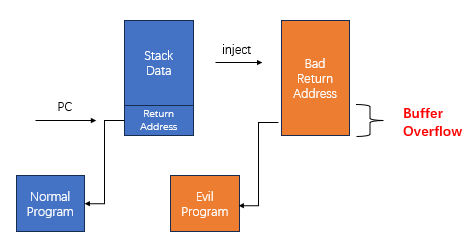
\includegraphics[width=0.5\textwidth]{pictures/Buffer Overflow.png}
		\caption{缓冲区溢出漏洞图示}
		\label{fig:UAF}
	\end{figure}
	
	攻击者可能利用缓冲区溢出漏洞来执行恶意代码,例如注入Shellcode并强制程序跳转到Shellcode的地址,从而获得系统权限。同时,也可能泄露敏感信息,例如通过溢出将重要的内存区域覆盖为攻击者所控制的数据,从而导致信息泄露。除此之外,因为缓冲区溢出可能导致程序崩溃或无法正常执行,使其无法提供正常的服务。
	
	著名的``Code Red''蠕虫利用了Microsoft
	IIS服务器上的缓冲区溢出漏洞。攻击者通过发送特制的HTTP请求,导致IIS的缓冲区溢出,并在受感染的系统上运行恶意代码。这导致系统被感染并且在网络上传播蠕虫。
	
\end{enumerate}

\subsubsection{模糊测试框架}
模糊测试(fuzzing)作为一种基于缺陷注入的自动化软件漏洞挖掘技术,是现在最有效的
漏洞挖掘技术。模糊测试向目标应用程序生成大量的正常和异常输入,并通过将生成的输入
提供给目标应用程序并监视执行状态来检测异常。与其他技术相比,模糊化易于部署,具有
良好的可扩展性和适用性,无论是否使用源代码,都可以执行。同时,由于模糊测试在代码
运行时进行监测,所以其具有较高的精度。

具体而言,模糊测试的工作过程包括四个主要阶段:测试样例生成阶段、测试样例运行阶
段、程序执行状态监控和异常分析阶段。模糊测试主要过程如图\ref{fig:fuzzing}所示。
\begin{figure}[ht]
	\centering
	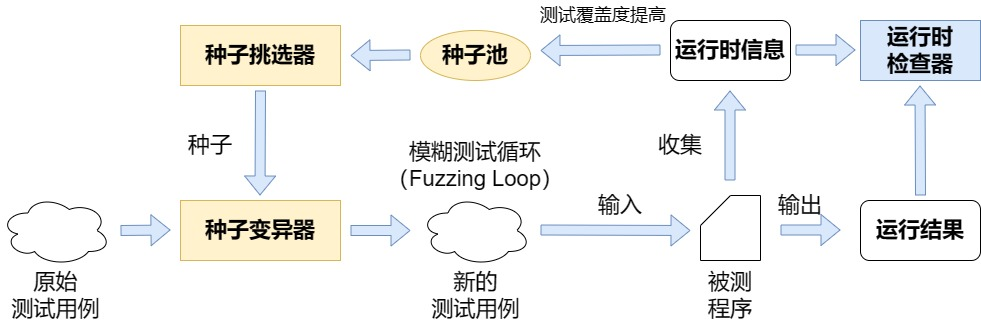
\includegraphics[height=4cm, width=13cm]{fuzzing.jpg}
	\caption{模糊测试流程图}
	\label{fig:fuzzing}
\end{figure}

模糊测试从生成测试用例开始,其生成的测试用例的质量直接影响模糊测试效果。其测试样
例一方面应满足测试程序对输入格式的要求,另一方面输入数据需要包含足够的异常数据,
以便这些输入在被程序处理时很可能导致程序失败或崩溃。根据目标程序的不同,输入可以
是具有不同文件格式的文件、网络通信数据、具有特定特征的可执行二进制文件等。如何生
成具有足够“破坏性”的测试用例是模糊器面临的一个主要挑战。一般来说,在现有的模糊器
中使用两种生成器,即基于生成的生成器和基于突变的生成器。

在前一阶段生成测试样例后,这些测试样例会被送入目标程序。模糊测试工具会自动启动并
结束目标程序的进程,并驱动目标程序的测试样例处理过程。在执行之前,分析人员可以配
置目标程序的启动和结束方式,并预定义参数和环境变量。通常,模糊测试过程会在预定义
的超时时停止,或是在程序执行挂起或崩溃时停止。

模糊测试工具在目标程序执行过程中监控执行情况,期待发现异常和崩溃。常用的异常监控
方法包括对特定系统信号、崩溃以及其他违规行为的监控。对于没有直观程序异常行为的违
规情况,可以使用许多工具,包括AddressSanitizer(Serebryany等,2012
年)、DataFlowsanitizer(The Clang Team,2017a)、ThreadSanitizer(Serebryany和
Iskhodzhanov,2009年)、LeakSanitizer(The Clang Team,2017b)等。当捕获到违规行
为时,模糊测试工具会存储相应的测试样例,以供后续重放和分析。在分析阶段,分析人员
尝试确定捕获的违规行为的位置和根本原因。分析过程通常借助调试器完成,比如
GDB、windbg,或其他二进制分析工具,如IDA Pro、OllyDbg等。二进制插桩工具,如Pin
等,也可以用来监控收集到的测试样例的确切执行状态,例如线程信息、指令、寄存器信息
等。自动崩溃分析是另一个重要的研究领域。

在执行完上述四个阶段之后,将根据程序反馈即代码覆盖率是否提升来判断种子是否有趣,
有趣的种子将被加入种子池中进行后续变异,进而形成新的测试样例重新输入待测程序。具
体而言,判断种子是否有趣的原则为选取开销小,作用大的种子,即如果两个种子可以得到
相同的代码逻辑覆盖情况,则保留文件较小的种子;如果两个种子可以得到相同的代码逻辑
覆盖情况,则选择耗时较小的。

根据程序源代码的依赖程度和程序分析的程度,模糊测试工具可以分为白盒、灰盒和黑盒。
白盒模糊测试假定能够访问程序的源代码,因此可以通过对源代码的分析以及测试用例如何
影响程序运行状态来收集更多信息。黑盒模糊测试在没有任何关于目标程序内部的知识的情
况下进行模糊测试。灰盒模糊测试也不需要源代码,通过程序分析来获得目标程序的内部信
息。

具体而言,白盒模糊测试是一种利用程序的内部结构和实现细节来生成测试用例的测试方
法。不同于黑盒模糊测试仅基于输入和输出进行测试,白盒模糊测试要求测试者对程序的内
部结构有深入了解。通过分析程序的源代码,白盒模糊测试使用符号执行和约束求解技术来
自动生成能够覆盖程序不同路径的输入数据,目标是深入程序内部逻辑以发现深层次的安全
漏洞和错误。

白盒模糊测试的一个核心特点是它的能力来处理高度结构化的输入,如编译器和解释器等应
用程序。这些应用程序按阶段处理输入,例如词法分析、解析和求值。白盒模糊测试结合了
静态分析和动态测试生成的方法,通过执行程序的符号执行并在此过程中生成和求解约束,
以自动化的方式生成测试输入。

白盒模糊测试在自动化测试生成、测试用例的执行以及测试结果的分析方面的广泛应用。这
包括但不限于利用程序分析技术优化测试过程、缩小输入空间、提高测试的自动化水平等。
白盒模糊测试通过这些技术手段实现了对复杂软件系统的有效测试,能够更加准确地发现并
定位软件中的安全漏洞和错误。

\subsubsection{ASan}

在模糊测试阶段自动分析运行时信息和输出结果时,程序会进行缺陷检测,而ASan(即
AddressSanitizer)是一种专为C和C++等编程语言设计的快速的内存错误检测工具,可以有
效地识别内存访问错误,包括堆、栈和全局变量的越界访问以及使用已释放堆内存
(use-after-free)的错误。具体而言,它采用了一种特殊的内存分配器和足够简单到可以
在任何编译器、二进制转换系统甚至在硬件中实现的代码插桩技术。ASan在不牺牲全面性的
情况下实现了高效率,其平均运行速度减慢仅为73\%,但它能够准确地在发生错误时立即检
测到错误。

ASan由两部分组成:一个插桩模块和一个运行时库。插桩模块修改代码以检查每次内存访问
的影子状态,并在栈和全局对象周围创建有毒的红色区域以检测溢出和下溢。当前的实现基
于LLVM编译器基础设施。运行时库替换了malloc、free及相关函数,围绕分配的堆区域创建
有毒的红色区域,延迟已释放的堆区域的重用,并进行错误报告。

从高层次上看,ASan对内存错误检测的方法与基于Valgrind的工具AddrCheck 类似:使用影
子内存记录每个应用程序内存字节是否安全访问,并使用插桩来在每个应用程序加载或存储
时检查影子内存。与之不同的是,ASan使用了更高效的影子映射、更紧凑的影子编码,在检
测堆外还能检测栈和全局变量中的错误,并且比AddrCheck快一个数量级。接下来将描述
ASan如何编码和映射其影子内存、插入其插桩,以及其运行时库如何操作。

\textbf{(一)影子内存}

malloc函数返回的内存地址通常至少对齐到8字节。这导致任何对齐的8字节序列的应用程序
堆内存都处于9种不同状态之一:前k个(0 $\leq$ k $\leq$ 8)字节是可寻址的,而剩下
的8 $-$ k字节则不是。这种状态可以编码成一个影子内存的单字节。

ASan将虚拟地址空间的八分之一专用于其影子内存,并使用一个比例和偏移的直接映射方式
来将应用程序地址翻译成相应的影子地址。给定应用程序内存地址Addr,影子字节的地址计
算为(Addr$>>$3)+Offset。如果$Max-1$是虚拟地址空间中的最大有效地址,那么Offset的
值应该选择为从Offset到$Offset+Max/8$的区域在启动时不被占用。在典型的32位Linux或
MacOS系统上,其中虚拟地址空间为0x00000000$-$0xffffffff, ASan使用Offset =
0x20000000 (2的29次方)。在一个具有47个有效地址位的64位系统上,我们使用Offset =
0x0000100000000000 (2的44次方)。在某些情况下(例如,在Linux上使用-fPIE/-pie编译
器标志),可以使用零偏移来进一步简化插桩。
\begin{figure}[ht]
	\centering
	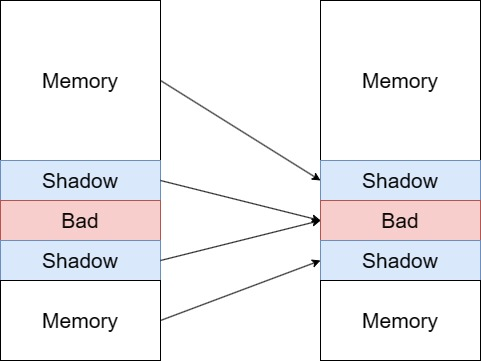
\includegraphics[height=9cm, width=13cm]{shadow.jpg}
	\caption{影子内存地址布局}
	\label{fig:shadow}
\end{figure}

图\ref{fig:shadow}展示了地址空间布局。应用程序内存被分为两部分(低和高),它们映射到相应的影子区域。将影子映射应用于影子区域中的地址会给我们在“坏”区域的地址,该区域通过页面保护标记为不可访问。

我们对每个影子字节使用以下编码:0意味着相应的应用程序内存区域的所有8字节都是可寻
址的;k(1 $\leq$ k$\leq$ 7)意味着前k个字节是可寻址的;任何负值表示整个8字节字
是不可寻址的。我们使用不同的负值来区分不同种类的不可寻址内存(堆红区、栈红区、全
局红区、释放的内存)。这种影子映射可以概括为形式(Addr$>>$Scale)+Offset,其中
Scale是1...7之一。当Scale=N时,影子内存占据虚拟地址空间的$1/2^N$,红区(以及
malloc对齐)的最小尺寸是$2^N$字节。每个影子字节描述了$2^N$字节的状态,并编码$2^N
+1$不同的值。更大的Scale值需要较少的影子内存但更大的红区来满足对齐要求。Scale值
大于3需要对8字节访问进行更复杂的插桩,但为可能无法放弃其地址空间连续八分之一的应
用程序提供了更多的灵活性。

\textbf{(二)插桩模块}

当对一个8字节的内存访问进行插桩时,AddressSanitizer计算相应影子字节的地址,加载
该字节,并检查它是否为零:

\begin{lstlisting}[language=C++]
ShadowAddr = (Addr >> 3) + Offset;
if (*ShadowAddr != 0)
ReportAndCrash(Addr);
\end{lstlisting}

当对1字节、2字节或4字节的访问进行插桩时,插桩过程会稍微复杂:如果影子值是正数
(即,8字节词中的前k个字节是可寻址的),我们需要将地址的最后3位与k进行比较。

\begin{lstlisting}[language=C++]
ShadowAddr = (Addr >> 3) + Offset;
k = *ShadowAddr;
if (k != 0 && ((Addr & 7) + AccessSize > k))
  ReportAndCrash(Addr);
\end{lstlisting}

在这两种情况下,插桩仅在原始代码的每次内存访问中插入一个内存读取。我们假设一个N
字节的访问是对齐到N的。ASan可能会错过由于未对齐访问引起的错误。

ASan的插桩阶段处在LLVM优化管道的最末端。这样我们只对那些经过LLVM优化器的所有标量
和循环优化后仍然存在的内存访问进行插桩。例如,通过LLVM优化掉的本地栈对象的内存访
问将不会被插桩。同时,我们不需要对LLVM代码生成器生成的内存访问进行插桩(例如,寄
存器溢出)。

\textbf{(三)运行库}

运行时库的主要目的是管理影子内存。在应用程序启动时,整个影子区域都会被映射,以便
程序的其他部分无法使用它。影子内存的坏段被保护起来。在Linux上,影子区域在启动时
总是未被占用的,因此内存映射总是成功的。在MacOS上,我们需要禁用地址空间布局随机
化(ASLR)。我们的初步实验表明,相同的影子内存布局也适用于Windows。

malloc和free函数被替换为特殊的实现。malloc函数在返回的区域周围分配额外的内存,即
红色区域(redzone)。红色区域被标记为不可寻址或“有毒”的。红色区域越大,将能检测
到的溢出或下溢也越大。

分配器内的内存区域被组织为一个自由列表数组,对应于一系列对象大小。当与请求的对象
大小相对应的自由列表为空时,将从操作系统(例如,使用mmap)分配一大组带有红色区域
的内存区域。对于n个区域,我们分配n + 1个红区,使得一个区域的右红区通常是另一个区
域的左红区:

\begin{figure}[ht]
	\centering
	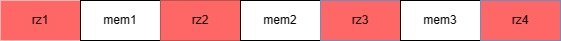
\includegraphics[height=1cm, width=15cm]{rz.jpg}
	\caption{红区分布}
	\label{fig:rz}
\end{figure}

左红区域用于存储分配器的内部数据(如分配大小、线程ID等);因此,堆红区的最小尺寸
当前为32字节。这些内部数据不会因为缓冲区下溢而被破坏,因为这种下溢会在实际存储之
前立即被检测到(如果下溢发生在被插桩的代码中)。

free函数将整个内存区域标记为有毒,并将其放入隔离区,以便这个区域在短期内不会被
malloc重新分配。目前,隔离区被实现为一个FIFO队列,随时持有固定数量的内存。

默认情况下,malloc和free记录当前的调用堆栈,以提供更多信息的错误报告。malloc调用
堆栈存储在左红区域(红区越大,可以存储的帧数就越多),而free调用堆栈存储在内存区
域的开始处。

为了检测对全局变量和栈对象的越界访问,ASan必须在这些对象周围创建有毒的红区。对于
全局变量,红区在编译时创建,并且红区的地址在应用程序启动时传递给运行时库。运行时
库函数将红区标记为有毒,并记录地址以供进一步的错误报告。

对于栈对象,红区在运行时创建并标记为有毒。目前,使用了32字节的红区(加上最多31字
节用于对齐)。例如,给定一个程序:

\begin{lstlisting}[language=C++]
void foo() {
	char a[10];
	<function body>
}
\end{lstlisting}

转换后的代码将类似于:

为了检测对栈对象的越界访问,AddressSanitizer对原有的函数foo进行了转换,增加了红
区(redzones)来围绕数组arr。这些红区在运行时被标记为“有毒”的,用于捕获任何对这
些区域的非法访问。下面是转换后的代码示例:

\begin{lstlisting}[language=C++]
void foo() {
	char rz1[32]; // 前红区
	char arr[10]; // 原始数组
	char rz2[54]; // 后红区,大小为32-10+32
	unsigned *shadow =
	(unsigned*)(((long)rz1>>8)+Offset);
	// 标记红区和数组周围为有毒
	shadow[0] = 0xffffffff; // rz1
	shadow[1] = 0xffff0200; // arr 和 rz2
	shadow[2] = 0xffffffff; // rz2

	// 函数体
	// 解毒所有区域
	shadow[0] = shadow[1] = shadow[2] = 0;
}
\end{lstlisting}

同时,ASan是线程安全的。影子内存只在相应的应用程序内存不可访问时被修改(在malloc
或free内部、在创建或销毁栈帧期间、在模块初始化期间)。所有其他对影子内存的访问都
是读操作。malloc和free函数使用线程局部缓存来避免每次调用都进行锁定(正如大多数现
代malloc实现所做的)。如果原始程序在内存访问和该内存的删除之间存在竞态,ASan有时
可能将其检测为使用后释放错误,但不能保证总能检测到。每次malloc和free的线程ID都被
记录,并在错误消息中与线程创建的调用栈一起报告。

\subsubsection{基于覆盖率的遗传算法}

基于代码覆盖率的遗传算法是一种将遗传算法原理应用于软件测试的方法,特别是在模糊测
试中,目的是通过优化测试用例来提高代码覆盖率,从而提升软件测试的全面性和效率。遗
传算法是受自然选择原理启发的优化技术,通过模拟生物进化过程中的选择、交叉(杂交)
和变异操作,来在解空间中搜索最优解。

具体而言,在进行模糊测试的过程中,程序通过代码覆盖率的高低来判断种子是否有趣。代
码覆盖率是一种简单的动态分析方法,常用于衡量测试的全面性。它通过将源代码分割成具
有一定粒度的“块”并追踪在运行时遇到了哪些块来实现。有时,还会记录在测试中遇到某个
特定块的次数。测量的覆盖率的粒度可以有所不同,并且存在多个定义来命名不同粒度,但
三种常用的定义包括块覆盖率、决策覆盖率和条件覆盖率。块覆盖率:在块覆盖率中,一个
块是指没有if语句或其他控制语句将执行从块中引导出去的代码片段。在运行时计算这些块
的覆盖率。决策覆盖率:决策覆盖率寻找应用程序做出决策的地方,主要是if语句,然后分
析所有可能的决策被覆盖得有多好。条件覆盖率:条件覆盖率也寻找if语句,并尝试追踪这
些分支中所有不同的布尔值是否已经被测试过。然而,如果应用程序的if语句包含多个条件
进行检查,条件覆盖率并不保证决策覆盖率。

基于代码覆盖率的遗传算法首先定义一个适应度函数来衡量测试用例的优劣,这里的适应度
函数即代码覆盖率。算法从一组测试用例开始,构成了初始种群。通过运行这些测试用例并
根据运行信息得到它们的代码覆盖率,以此来评估种群中每个个体的适应度。并将产生的适
应度高的新测试用例替换种群中适应度较低的测试用例。重复上述步骤,直到达到预定的迭
代次数或代码覆盖率达到预期水平。

基于代码覆盖率的遗传算法在模糊测试中起着非常重要的作用,它可以自动化地生成能够触
发新路径的输入,为软件安全和质量提供了一个强大的工具。通过不断地迭代和优化,这种
方法能够有效地提升测试的深度和广度,帮助开发识别和修复软件中的漏洞。


%author: yjw, 2024-4-1
\subsubsection{ROS2系统机制}
在 ROS 2的体系结构中,节点(Node)是最基本的执行单位,负责特定功能的实现,如数据
处理或硬件接口。每个节点可以包含多种通信机制,包括订阅者(Topic Subscribers)、
定时器(Timer)、服务服务器(Service Servers)和服务客户端(Service Clients),
如图\ref{pic:rns}。这些通信实体的目的是为了接收和发送数据,以及提供不同的服务。

节点注册到执行器(Executor)中,执行器是一个控制实体,负责协调节点的活动。当节点
的一个通信事件发生时,比如收到一个主题消息或服务请求,执行器会调用相应的处理函
数,或称为回调函数(Callback)。这些回调函数是预先定义的,用来响应特定类型的事
件,如 \texttt{topic\_receive()} 用于处理主题消息, \texttt{request\_receive()}
用于处理服务请求,\texttt{time\_up()}用于处理定时器完成计时。

在节点的生命周期中,可以使用生命周期状态机(Lifecycle SM)来管理节点的状态,这在
管理复杂节点时特别有用。生命周期状态机允许节点在不同状态之间转换,如激活
(activate)、去激活(deactivate)和清理(cleanup)。每个状态变化都可以有对应的
回调函数,例如\texttt{setting()}在节点激活时调用,用于声明节点接口、节点执行器
(Executor)、通信订阅和服务订阅等一系列节点功能实体;\texttt{activate()} 用于节
点初始化完毕开始服务,此时节点处于正常工作状态; \texttt{cleanup()}在节点清理资
源时调用,用于释放节点所持有的微机资源。

\textbf{ROS2事件处理机制}: 

节点调用 \texttt{spin()} 函数来持续检查和处理事件,如伪代码\ref{lst:rosspin}。

\begin{figure}[H]
\begin{lstlisting}[language=Python]
spin():
    while True:
        new_msg <- ros_dds_listener()
        handler <- get_callback(new_msg)
        Executor.execute(*handler)
        sleep(0.1)
\end{lstlisting}
\caption{ROS2事件循环示例}
\label{lst:rosspin}
\end{figure}

\texttt{spin()} 实质是一种事件循环,它会保持节点循环和监听,检查系统中是否有新的
ROS消息或待处理的消息,获取到消息实体后,根据消息类型获取节点初始化时注册的回调
函数,交付给节点执行器去执行,从而完成对该事件(消息)的响应。 \texttt{spin()}函
数是一个事件循环,保持节点持续运行并响应事件。

在执行器内部,\texttt{execute\_any\_*()} 函数是对ROS核心细节的抽象,这个函数根据
事件的类型和优先级选择一个事件来处理。处理过程包括执行注册的回调函数,这些函数是
在节点初始化时注册的,如\texttt{timer.registe\_handler()}用于注册定时器事件的回
调;\texttt{subscriber.regeste\_handler()} 用来注册监听到某话题时触发的回调函
数,以处理该数据。

总体而言,ROS2的程序机制基于事件驱动的模型,通过节点、执行器和回调函数协同工作来
响应和处理各种事件,这些事件可能来源于数据的接收、定时器的触发、服务的请求和响
应,以及节点生命周期状态的变化。通过这种灵活且模块化的设计,ROS 2能够支持复杂且
多样化的机器人系统开发。


\begin{figure}[H]
    \centering
    \includegraphics[width=15cm]{ros_node_setup.png}
    \caption{ROS节点内部模型, 初始阶段}
    \label{pic:rns}
\end{figure}

\textbf{ROS2节点释放}

当ROS2系统的节点将释放时,节点的生命周期状态机会从 activate 状态转换为
deactivate 状态,此状态仅用于让节点完成必要的最后工作,如完成正在处理的数据传输
或请求,然后进入非活跃状态。

紧接着,节点生命周期状态机转为 cleanup 状态,见图\ref{pic:rnc},调用
\texttt{cleanup()} 回调函数来释放节点拥有的资源,这包括所有回调函数(callback
handlers),如和话题订阅、定时器、服务等回调函数。然后清理节点所打开的文件,断开
网络连接,释放ROS2上下文,最终释放内存。

\begin{figure}[H]
    \centering
    \includegraphics[width=15cm]{ros_node_cleanup.png}
    \caption{ROS节点内部模型, 释放阶段}
    \label{pic:rnc}
\end{figure}

\textbf{ROS2通信机制}

为了适应机器人系统中复杂的通信需求,ROS2设计了一套专用的通信模型。其基础为“发
布、订阅“模型,支持节点间的异步数据交换。该机制允许ROS2系统内的节点(Node)独立
地发布(Publish)和订阅(Subscribe)消息,而不需要彼此之间的直接连接或相互了解。
这种设计显著提高了系统的灵活性和扩展性,因为它允许任何数量的发布者和订阅者存在于
同一个话题上,从而实现了高效的多对多通信。

在ROS 2的架构中,每个节点可以根据其功能需求,声明为发布者或订阅者,类似图
\ref{pic:rmp},或同时充当这两种角色。发布者负责生成并发布特定类型的消息到一个命
名的话题上,而订阅者则监听这个话题,接收并处理传入的消息。监听到并处理消息时,使
用的是订阅该话题时传入的回调函数来自动处理,订阅者不必同步阻塞就能等待处理订阅消
息。话题本质上是一个数据通道,它通过唯一的名称标识,确保消息的传递和接收的一致
性。每个话题都与一个明确的消息类型相关联,这个消息类型使用YAML格式定义各字段的静
态变量类型,从而定义了该话题传输数据的结构。

此通信机制的一个核心优点是其异步性,使得发布者和订阅者可以独立地操作,增加了处理
并发消息的能力。此外,由于发布者和订阅者之间的解耦,系统组件可以被设计得更为模块
化,易于开发和维护。例如,在自动驾驶的应用场景中,激光雷达传感器节点可以发布其测
量到的数据到话题 \textbackslash scan,而负责建图和规划路径的节点则通过订阅该话题
来实时获取雷达信息,从而完成最终决策。


\begin{figure}[H]
    \centering
    \includegraphics[width=13cm]{ros_msg_passing.png}
    \caption{ROS话题通信机制}
    \label{pic:rmp}
\end{figure}

\textbf{ROS2 通信机制底层实现}

ROS2通信机制底层实质是使用UDP Socket来进程间通信,使用的协议为物联网DDS协
议,ROS2核心库对其进行了抽象封装,已便捷地被开发者调用。具体而言,对于每种DDS协
议版本,ROS2会实现一种网络中间件对其API进行包装,并实现由ROS2各类消息形式向DDS消
息格式的序列化与结构化转化。如图\ref{pic:rmpm}

\begin{figure}[H]
    \centering
    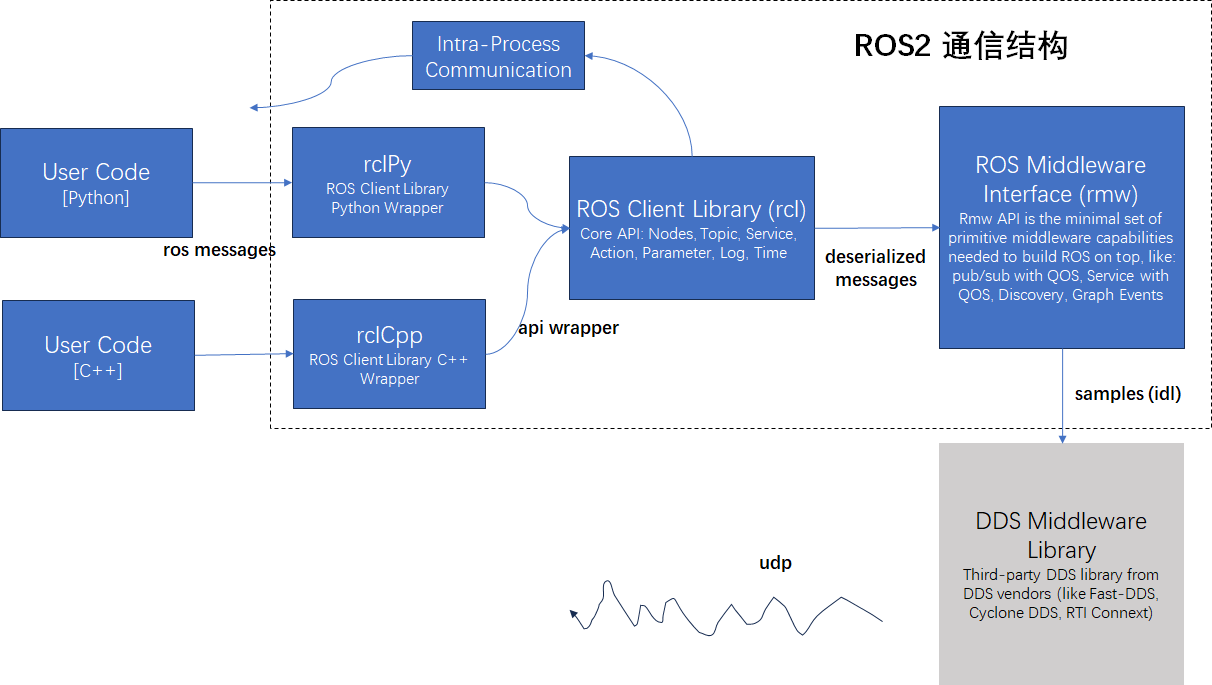
\includegraphics[width=13cm]{ros_msg_passing_mdw.png}
    \caption{ROS底层通信机制实现}
    \label{pic:rmpm}
\end{figure}

\subsection{关键设计} %@author: yjw
%author: yjw, 2024-4-1
%\subsection{关键设计}
\subsection{系统需求分析}
\setParDis %设置段间距为 0
%@author: wkt
\begin{enumerate}
  \item 高覆盖率
  \item 高效性快速收敛
  \item 可拓展性
  \item 准确性高
\end{enumerate}
本项目核心目标是将自动模糊测试(Fuzzing)框架迁移到ROS2系统上,并且针对ROS2特性
对测试效率做出改进提升。具体而言,我们试图寻找更多可能的程序输入口,使测试覆盖的
输入可能性尽可能多;尝试构造质量尽可能高的初始种子;寻找更多反馈信息,用于监控被
测程序(即ROS2节点)的内部状态,以更高效地指导对输入的变异;尝试模拟更多ROS2执行
环境,模拟程序可能遇到的各种实际情况。

\subsubsection{通信环境测试}

\begin{figure}[h]
    \centering
    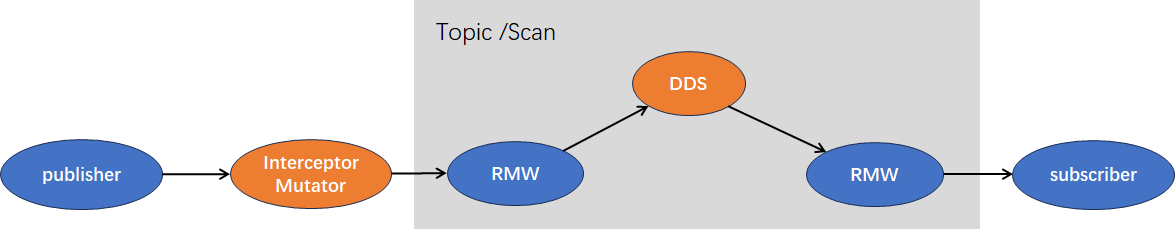
\includegraphics[width=15cm]{fuzz_msg_passing.png}
    \caption{ title}
    \label{pic:fmp}
\end{figure}

\begin{figure}[h]
    \centering
    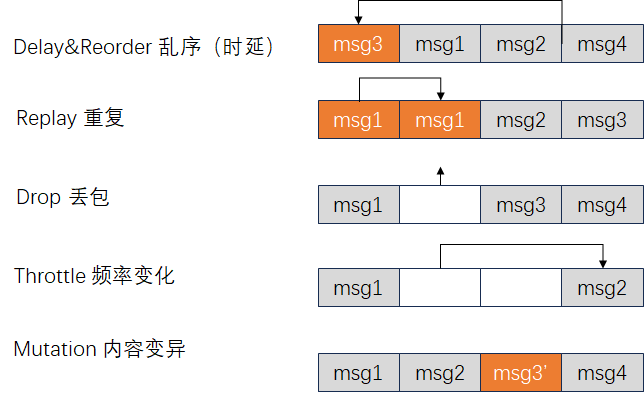
\includegraphics[width=10cm]{fuzz_msg_mutation.png}
    \caption{ title}
    \label{pic:fmm}
\end{figure}

\subsubsection{多维度输入}

\begin{figure}[h]
    \centering
    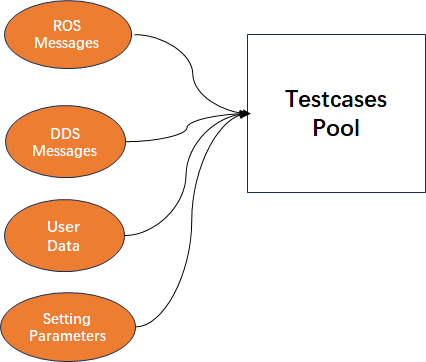
\includegraphics[width=7cm]{fuzz_multi_input.png}
    \caption{ title}
    \label{pic:fmi}
\end{figure}

$^{[2]}$, 

\subsubsection{基于延迟插入的并发漏洞检测}

\begin{figure}[h]
    \centering
    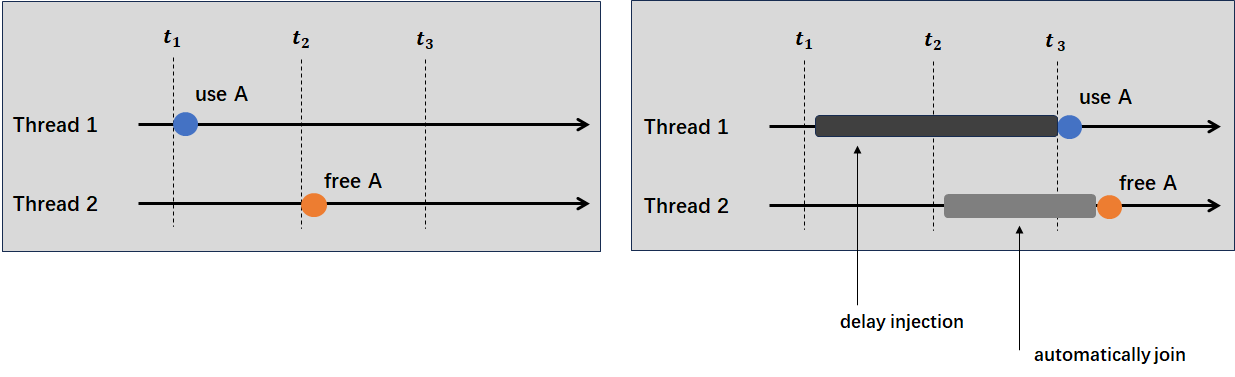
\includegraphics[width=15cm]{fuzz_delay_injection.png}
    \caption{ title}
    \label{pic:fdi}
\end{figure}

\begin{figure}[h]
    \centering
    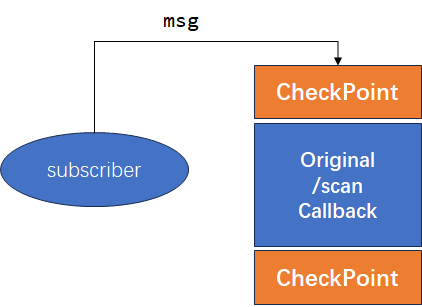
\includegraphics[width=7cm]{fuzz_instrumentation.png}
    \caption{ title}
    \label{pic:fi}
\end{figure}

$^{[1]}$, 

\subsubsection{测试反馈}
\begin{figure}[h]
    \centering
    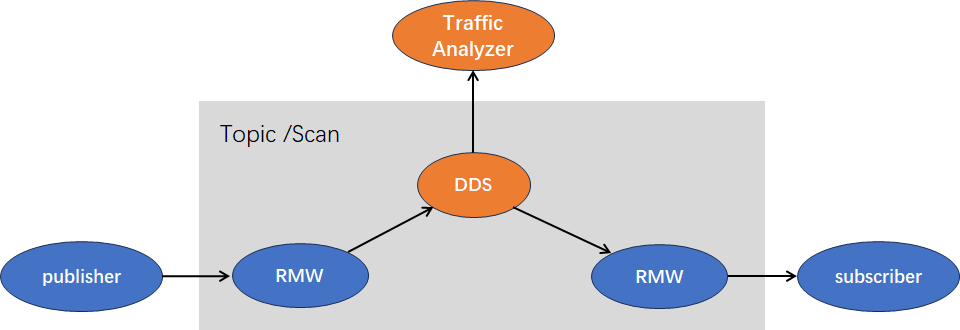
\includegraphics[width=15cm]{fuzz_traffic_monitor.png}
    \caption{ title}
    \label{pic:ftm}
\end{figure}
\subsubsection{测试加速}



%********************* 三 成果与分析 *****************
\section{作品测试与成果分析} %@author: wkt
\setParDis %设置段间距为 0

\subsection{测试环境介绍}
本作品在ROS2中测试了10个常见的机器人程序。根据最新版本的测试结果得到下列图表,表
格\ref{tb:ros_test}显示了这些用于测试的ROS程序的信息(LOC指代码行数)。为了执行机
器人导航(用于移动和定位程序)和地图构建(用于移动和SLAM程序)任务,这些程序在机器人
仿真框架Gazebo11.5$^{[4]}$中的虚拟机器人TurtleBot3 Waffle上执行。本测试使用的虚
拟传感器包括激光雷达,里程计,2D相机和IMU(惯性测量单元)。实验运行在一台x86-64台
式机上,配有32个Intel处理器核心和64GB物理内存。使用的操作系统为Ubuntu 22.04,
ROS2版本为ROS2 Humble。
\begin{table}[H]
	\small
	\caption{用于测试的ROS程序信息}
	\label{tb:ros_test}
	\centering
	\begin{tabular}{cccc}
		\hline  
		\textbf{类型} & \textbf{程序} & \textbf{描述} & \textbf{LOC} \\ 
		\hline  
    导航 & navigation2 & ROS2导航系统 & 25.8K \\
		定位 & nav2\_amcl & ROS2导航中的定位模块 & 14.4K \\
		定位 & lama\_loc & 可选的定位和映射方法 & 9.5K \\
		定位 & ekf\_loc & 基于卡尔曼滤波的定位方法 & 0.8K \\
		建图 & rtab-map & 实时RGB-D SLAM方法 & 26.1K \\
		建图 & slam\_toolbox & 一套用于2D SLAM的工具和功能 & 15.1K \\
    底层 & ros2rclcpp & ROS2底层基础设施 & 177.1K \\
		\hline
	\end{tabular} 
\end{table}

\subsection{测试成果与漏洞统计}
在作品开发过程中,我们对上述项目进行了广泛测试,表格\ref{tab:test_result}显示了
截稿时的漏洞发掘结果。

\begin{table}[H]
	\small
	\caption{机器人程序在ROS2模糊测试结果}
  \label{tab:test_result}
	\centering
	\begin{tabular}{ccccc}
		\hline
		\textbf{程序} & \multicolumn{2}{c}{\textbf{覆盖分支}} & \multicolumn{2}{c}{\textbf{漏洞检测}} \\
		\cline{2-5}
		& \textbf{模糊测试} & \textbf{测试样例} & \textbf{发现的漏洞} & \textbf{受修复漏洞} \\
		\hline
		navigation2 & 37.6K & 36.8K & 12 & 8 \\
		lama\_loc & 20.8K & 20.7K & 2 & 0 \\
		ekf\_loc & 3.3K & 5.4K & 1 & 0 \\
		rtab-map & 70.9K & 59.3K & 3 & 1 \\
		slam\_toolbox & 12K & 10.7K & 3 & 2 \\
		cartographer & 51.9K & 52.1K & 4 & 0  \\
    rclcpp & None & 47.2K & 3 & 0 \\
		\textbf{总计} & None & None & 28 & 11 \\
		\hline
	\end{tabular}
\end{table}

\textbf{测试覆盖率。}本作品初始输入样例(即未经过自动生成的初始测试输入)包含了
官方的测试用例,但基于这部分测试样例并没有发现新的漏洞,对代码覆盖率贡献也较低,
侧面反映了传统测试用例的低效性。本作品能否稳定提高开源程序测试代码覆盖率,部分项
目由于多版本问题覆盖率才略低于官方测试样例。

\textbf{漏洞检测。本作品在测试程序中发现了28个真实的漏洞,并提供了稳定的复现办
法。本团队已经向相关ROS开发者报告了这些漏洞,其中活跃项目(如navigation2)中11个
漏洞已经得到了确认和修复,部分低活跃程序仍在等待回复。其中Navigation2项目中4个危
险漏洞被美国通用漏洞披露库(CVE)收录,这充分证明了本作品检测出的漏洞的价值。}

\subsection{ROS漏洞实例分析}
% 2024-04-03
% author: yjw

下面挑选我们的漏洞测试系统在ROS相关项目中检测出的几个典型漏洞进行分析,它们充分
体现了本系统的价值。在Navigation2 Issue\#4177中,我们指出了一个典型的数组越界漏
洞。

Navigation2 系统中的节点会监听 \texttt{\textbackslash costmap},来更新代价地图信
息,但是缺乏对代价地图信息合法性的检查。如代码段\ref{lst:bug:msg}中的map消
息,width和height字段指出了代价地图的宽高,data字段给出了代价地图的数据。对于正
常消息,$width\times height$应该等于data数组的大小,但这一点对于传输错误或恶意投
放的消息这并不是被严格保证的。

\begin{figure}[H]
\begin{lstlisting}[]
ros2 topic pub /map nav_msgs/msg/OccupancyGrid "
...
info:
  ...
  width: 2
  height: 2
  ...
data: [-1, 0, 1, 1, -1]  " <- would cause buffer overflow
\end{lstlisting}
  \caption{漏洞\#4177恶意消息}
\label{lst:bug:msg}
\end{figure}

Navigation2 自动导航项目并没有对这一点进行检查,而直接用width和height声明存储
data的数组变量。当\texttt{width}和\texttt{height}大于数组\texttt{data}的实际大小
时,会导致程序访问越界(SEGV)。初始化地图时该bug可能触发,见代码段
\ref{lst:bug:segv}第6行;运行时,如果接收到外部更新的地图信息,也可能触发该问
题,见代码段\ref{lst:bug:segv}第24行。

\begin{figure}[H]
\begin{lstlisting}[language=C++]
/* 初始化时可能发生 */
// create the costmap
costmap_ = new unsigned char[size_x_ * size_y_];
for (unsigned int it = 0; it < size_x_ * size_y_; it++) {
  data = map.data[it]; // <- SEGV
  if (data == nav2_util::OCC_GRID_UNKNOWN) {
    costmap_[it] = NO_INFORMATION;
  } else {
    ...
  }
}

/* 过程中也可能发生,比如接收到外部更新的地图信息 */
void CostmapSubscriber::toCostmap2D()
{
  auto msg = std::atomic_load(&costmap_msg_);
	...
  unsigned char * master_array = costmap_->getCharMap();
  unsigned int index = 0;
  for (unsigned int i = 0; i < msg->metadata.size_x; ++i) {
    for (unsigned int j = 0; j < msg->metadata.size_y; ++j) {
      master_array[index] = msg->data[index]; //<-SEGV
      ++index;
    }
  }
}
\end{lstlisting}
  \caption{漏洞\#4177问题代码}
\label{lst:bug:segv}
\end{figure}

在Naviagtion2PR\#3972, PR\#3958, Issue\#3940$^{[13]}$中,我们报告了一个典型的并发
bug,本系统通过插桩延迟技术,找到了Navigation2项目中Costmap结构数据竞争的根本原
因,删除了之前大量不必要的检查。

此bug发生在关闭期间,ROS系统使用Lifecycle状态机机制来管理节点生命周
期,Controller、Planner、 CostmapROS都是具有生命周期的节点,CostmapROS是
Controller和Planner的子节点(独立线程)。当ROS2系统关闭时,Lifecycle状态机发送同
一关闭信号,这三种节点都会直接对该信号进行响应然后执行资源释放程序,此时三者关闭
顺序是不一致且不确定的。

如果子线程CostmapROS节点已经自行释放,Controller或Planner实质失去了对其的控制
权,如果它们仍试图访问CostmapROS,就产生了重复释放(UAF)、资源冲突等一系列并发
问题,如伪代码\ref{lst:bug:issue3972}所示。

\begin{figure}[H]
\begin{lstlisting}[language=C++]
// Planner or Controller:
Controller::on_cleanup(const rclcpp_lifecycle::State &){
	costmap_ros_->cleanup() // <-UAF, costmap already cleanup itself.
}
\end{lstlisting}
  \caption{漏洞\#3972问题代码}
  \label{lst:bug:issue3972}
\end{figure}

对于需要频繁开关的机器人节点,关闭期间内存漏洞可能产生严重后果,但往往被开发者忽
略。在 Navigation2 Issue\#4175,PR\#4180,Pull\#4176,和 RclCpp Issue\#2447
$^{[14]}$ 中,我们和ROS2开发者讨论了ROS2节点退出机制可能导致的一些并发问题。

ROS2惯例是将收到订阅消息、收到服务请求的回调函数交给执行器(Executor)执行,因此
执行器线程拥有该回调函数的函数指针,当该回调函数所属的类已被释放,如伪代码
\ref{lst:bug:issue4176}第5行,执行器仍可能访问该回调函数,造成UAF错误。

\begin{figure}[H]
\begin{lstlisting}[language=C++]
nav2_util::CallbackReturn
AmclNode::on_cleanup(const rclcpp_lifecycle::State & /*state*/){
  ...
  initial_pose_sub_.rest(); // <- UAF
  
  ...
  executor_thread_.reset();
}

\end{lstlisting}
  \caption{漏洞\#4176问题代码}
  \label{lst:bug:issue4176}
\end{figure}



% 下面是原论文的ROS漏洞实例分析
本团队还根据发现的28个漏洞的类型进行了分类,并将结果总结在表
\ref{tab:test_bug_types}中。具体来说,有7个并发类型漏洞(包括数据竞争和少数死
锁),7个释放后使用错误(UAF),3个缓冲区/堆栈溢出错误,3个无效指针访问(SEGV)
和8个未捕获异常。一旦这些错误被特定的输入触发,运行时故障和严重安全问题就会发
生,严重威胁机器人的安全性和可靠性。

\begin{table}[H]
	\small
	\caption{发现漏洞的种类}
  \label{tab:test_bug_types}
	\centering
	\begin{tabular}{ccccccc}
		\hline
		\textbf{程序} & \textbf{数据竞争/死锁} & \textbf{UAF} & \textbf{溢出} & \textbf{SEGV} & \textbf{未捕获异常} & \textbf{总计} \\
		\hline
		navigation2 & 1 & 4 & 3 & 2 & 2 & 12\\
		lama\_loc & 2 & 0 & 0 & 0 & 0 & 3 \\
		ekf\_loc & 0 & 0 & 0 & 0 & 1 & 1 \\
		rtab-map & 0 & 0 & 0 & 1 & 2 & 3 \\
		slam\_toolbox & 2 & 1 & 0 & 0 & 0 & 3 \\
		cartographer & 1 & 0 & 0 & 0 & 3 & 4 \\
    rclcpp & 1 & 2 & 0 & 0 & 0 & 3\\
		\textbf{总计} & \textbf{7} & \textbf{7} & \textbf{3} & \textbf{3} & \textbf{8} & \textbf{28} \\
		\hline
	\end{tabular}
\end{table}

内存安全错误,如UAF、BufferOverflow、SEGV,由于易被攻击者利用和植入恶意程序,往
往更受开发者关注,但尽管如此,超过一半的漏洞威胁仍属于内存安全。由于机器人和自动
驾驶相关项目的应用特殊性,程序异常应给予日志记录而不应直接造成程序异常终止;但由
于复杂开源项目的异常处理管理难度大,常常出现开发者间合作不慎而导致异常未被捕获的
情况,底层开发者可能认为应用层开发者会处理该异常,而顶层开发者却可能也认为底层开
发者已经处理了此异常情况。部分UAF漏洞也可能由数据竞争等并发漏洞引发,部分数据竞
争漏洞大部分时间可能不会影响程序运行,造成隐蔽性极高,开发者确认和修复难度也大;
相反,死锁等阻塞型漏洞,通常由于错误使用ROS2通信机制导致,但容易修复和确认。

% 本测试检测到的5个释放后使用漏洞是由数据竞争引起的。具体来说,一个内存对象在一个线程中被释放,但这个对象仍然在另一个线程中使用,没有同步。由于并发执行的不确定性,在正常执行中很难发现这些漏洞。一个真实含有释放后使用漏洞的代码如图表1所示

% 本测试检测到的这18个未捕获的异常中,有8个错误是由被测程序代码中的内部异常引起的,10个错误是由被测ROS程序使用的第三方软件库和ROS核心组件的API调用的外部异常(在c++中属于``运行时错误''类型)引起的。这个特性表明应该在ROS程序中小心地捕获和处理内部和外部异常。例如,在nav2\_bt\_navigator、nav2\_planner、nav2\_controller和nav2\_amcl中,没有捕捉到来自ROS
% rclcpp组件的关于负时间间隔的四个外部异常,这可能导致程序崩溃。真实的代码案例如下图表2所示:

% 在ROS程序初始化过程中出现了11个bug。这些错误中有6个是由于初始化过程中对无效用户数据和不正确参数配置的错误处理引起的;还有5个漏洞是由初始化过程和消息处理之间缺少同步引起的。因此,在测试ROS程序时,应该特别注意初始化过程。

% 通过手工检查发现漏洞的回溯,本团队发现有7个漏洞位于被测试的ROS程序所使用的第三方库和ROS核心组件中。这些库和组件包括libopencv、fasttps、eigen、tf2和rclcpp。由于在实验中使用Asan仅仅检测被测试的ROS程序,而不是这些库或组件,因此无法找到这些漏洞的准确位置。为了解决这些问题,本作品尝试使用ASan来检测这些库和组件。但在尝试中发现,它们都不能支持ASan。即便如此,本团队在不使用ASan的情况下手动检查源代码并且成功在rclcpp中找到了一个漏洞(堆栈溢出)。目前rclcpp开发人员已经确认并修复了这个漏洞。

% 7个漏洞是由回调函数的并发性引起的。在ROS程序中,外部事件(如消息到达)随时会发生,并且每种事件均是由回调函数处理。由于事件可以在任何时间发生,它的回调函数可以与其他函数并发执行。因此,由于不正确的同步,回调函数中可能出现并发错误。图6(a)显示了nav2\_planner中的一个示例错误。回调函数footprint.callback可以与函数getFootprint并发执行。在footprint.callback函数中,指针footprint\_与msg在第106行一起被分配,因此由footprint\_所指向的内存会根据智能指针的功能被释放。同时,getFootprint中仍然使用这个智能指针来访问第76行中的footprint\_-\textgreater polygon,因此导致释放后使用的漏洞。{[}35{]}

% 11个漏洞是由错误处理问题引起的。具体来说,其中6个错误是由于对无效用户数据和错误的配置参数缺少或不正确的安全检查而引入的;另外5个错误是由于正确的安全检查后错误处理不正确而引入的。图6(b)显示了nav2\_controller中的一个示例错误。transformLaserScanToPointCloud函数可以在运行时抛出一个显式异常和一个隐式异常。在第294行只捕获显式异常,但未捕获``运行时错误''类型的隐式异常{[}36{]}。

% 2个漏洞是由堆栈内存问题引起的。其中一个漏洞是由在新线程中使用局部变量引起的,另
% 一个漏洞是由过多的递归调用引起的。图6(c)显示了rtab-map中的一个示例错误。在
% CoreWrapper类的构造函数中,主线程的第141行定义了一个局部变量tfDelay,但是这个变
% 量是在一个通过new std::thread创建的新线程中的第590行被访问的。由于新线程无法访问
% 主线程的堆栈,因此会出现堆栈溢出错误{[}37{]}。

% \subsection{与同类技术对比}
% 本测试通过实验将本作品与两种最先进的机器人程序测试方法Ros2-fuzz$^{[10]}$和
% ASTAA{[}38{]}进行了比较。ROS2 -fuzz是一种基于AFL$^{[11]}$的自动化模糊测试方法,
% 用于在ROS2中测试机器人程序。这种方法会对给定ROS节点中特定主题的消息进行变异。由
% 于Ros2-fuzz是开源的,我们从源代码构建它。ASTAA是一种针对机器人程序鲁棒性测试的方
% 法。它在ROS节点之间随机改变消息,并且还可以在运行时丢弃一些消息以模拟通信不稳
% 定。由于ASTAA是闭源的,本团队通过修改本作品实现了一个类似ASTAA的工具,只允许传感
% 器消息的数据突变和随机丢弃消息,而不使用程序反馈。

% 在实验中,我们在表1中选择了5个名称包含``nav2''的程序,并运行Ros2-fuzz、ASTAAlike
% 工具和本作品对这些程序进行了24小时的机器人导航任务测试。表4显示了比较结果,其中
% 包括覆盖的代码分支和发现的漏洞。
% \begin{table}[H]
% 	\small
% 	\caption{不同测试方法的漏洞检测结果}
% 	\centering
% 	\begin{tabular}{ccccccc}
% 		\hline
% 		\multirow{2}{*}{\textbf{程序}} & \multicolumn{2}{c}{\textbf{Ros2-fuzz}} & \multicolumn{2}{c}{\textbf{ASTAA-like}} & \multicolumn{2}{c}{\textbf{本作品}} \\
% 		\cline{2-7}
% 		& \textbf{分支} & \textbf{发现漏洞数} & \textbf{分支} & \textbf{发现漏洞数} & \textbf{分支} & \textbf{发现漏洞数} \\
% 		\hline
% 		nav2\_bt\_navigator & 1.8K & 0 & 23.7K & 1 & 24.3K & 3 \\
% 		nav2\_planner & 1.6K & 0 & 26.4K & 2 & 27.9K & 6 \\
% 		nav2\_recoveries & 4.8K & 0 & 15.1K & 1 & 15.8K & 2 \\
% 		nav2\_controller & 3.1K & 0 & 35.2K & 3 & 37.6K & 3 \\
% 		nav2\_amcl & 0.7K & 0 & 11.9K & 2 & 12.2K & 9 \\
% 		\textbf{总计} & \textbf{12.0K} & \textbf{0} & \textbf{112.3K} & \textbf{9} & \textbf{117.8K} & \textbf{23} \\
% 		\hline
% 	\end{tabular}
% \end{table}
% 本作品发现了Ros2-fuzz和ASTAA-like的工具发现的所有9个漏洞,并且它还发现了这些方法遗漏的14个漏洞,且具有更高的代码覆盖率。实际上,Ros2-fuzz和ASTAA仅生成关于ROS节点之间消息的测试用例,因此在模糊测试期间没有涉及处理不同用户数据和配置参数的大量代码。相比之下,本作品从多个维度(包括用户数据、配置参数和传感器消息)生成测试用例,因此本作品覆盖了Ros2-fuzz和ASTAA遗漏的更多代码。此外,本作品使用分布式分支覆盖更有效地指导多个ROS节点的测试用例生成,并使用三种常见模式执行时间突变(ASTAA只考虑其中一种模式,即消息丢弃),以更有效地覆盖有关时间特征的代码。由于这些原因,在实验中,本作品比Ros2-fuzz和类ASTAA-like的工具产生更好的结果。

% 通过分析被覆盖分支随着测试时间的增长,观察到随着时间的推移,这三种工具覆盖的新代码分支越来越少。这是因为许多代码分支已经被模糊测试期间由早期突变生成的测试用例所覆盖。即便如此,本团队观察到在后面的测试中,由于本项目的多维生成方法、分布式分支覆盖和时间突变策略,本作品覆盖了更多的新代码分支。

% 创新型说明与前景分析 @author: jfb
% author: jfb
\subsection{创新性说明}
%TODO @jfb, 请将wkt1.tex和这部分的创新型结合总结一下
\textbf{创新地将模糊测试技术迁移}
  
本作品创新性的将模糊测试迁移到了ROS框架中来,拓展了传统软件测试方法的应用范
围,这一创新性的做法为机器人系统安全性和鲁棒性的提升开辟了新的途径。特别是在自
动驾驶车辆、工业及服务机器人等领域,安全性是至关重要的。通过针对ROS系统特有的
模块化和分布式架构进行定制化的模糊测试,不仅能有效发现和修复潜在漏洞,提高系统
对异常输入的处理能力,还能增强系统面对复杂物理环境的稳定性。

此外,这种方法的引入,促进了ROS社区对安全问题的广泛关注,有助于建立更安全的ROS
生态系统。同时,这也为机器人软件测试领域带来了新的测试工具和思路,给机器人软件
开发中测试和验证方法的重要进步。总的来说,将模糊测试技术应用于ROS框架,不仅为
机器人系统的安全性和稳定性提供了强有力的支持,也为机器人软件测试和验证方法的创
新开辟了新的方向。
  
\textbf{创新测试方法,高效性}
  
本作品相较于传统的软件测试方法,有效提升了代码的测试的覆盖率与准确率的同时,运
行效率也实现了大幅度提高。本作品能也成功发现数十个被常规测试方法忽略的隐蔽漏
洞,特别是那些与安全高度相关的漏洞,如缓冲区溢出、内存泄露等。由于其自动化特
性,大大提高了测试效率。

此外,模糊测试易于集成进现有的开发和测试流程,尤其是与持续集成系统相结合时,可
以实现持续的安全监测,进一步减少安全漏洞带来的风险。通过在软件发布前发现并修复
潜在的安全问题,模糊测试有助于减轻安全事故的风险,保护企业和用户的数据安全,同
时节省潜在的调查、修复和法律相关的成本,展现出其良好的成本效益比。这些优势共同
促进了模糊测试成为提高软件安全性和可靠性的重要工具。
    

本作品的核心模糊测试程序优势如下: %TODO @jfb,这部分请和前一部分融合一下
\begin{enumerate}
	\item 高覆盖率 \\
	ROS系统的架构复杂,包含多个节点和话题,而本作品能够系统性地探索这些节点和话题之间的交互,从而实现全面覆盖。通过生成各种可能的输入和交互序列,本作品能够有效地发现潜在的漏洞和异常情况,为系统的安全性和稳定性提供保障。例如,它可以模拟不同的传感器输入和控制命令,以验证ROS系统对于各种情境的响应是否符合预期,从而增强系统的健壮性和可靠性。
	通过分布式分支覆盖,它能够捕获不同节点之间的代码执行路径,从而更全面地测试机器人程序。
	本作品使用多维生成方法生成ROS程序的测试用例,包括用户数据、配置参数和传感器消息。这种方法有助于覆盖不同维度的输入空间,提高测试的全面性。
	\item 高效性快速收敛 \\
	通过自动化生成和执行测试用例,本作品大幅提高了测试效率。快速生成大量测试用例,并采用智能化的测试执行策略,使得工具能够在短时间内快速收敛到潜在问题,帮助开发人员及时发现和修复bug,从而提高开发周期效率。举例来说,本作品可以根据程序执行路径的优先级和覆盖情况,动态调整测试用例的生成和执行顺序,优先测试具有潜在问题的部分,从而更快地发现关键问题。
	\item 可拓展性 \\
	由于ROS系统的多样性和复杂性,模糊测试工具必须具备良好的可拓展性,以应对不同类型和规模的ROS应用。这种工具通常设计成模块化的结构,能够轻松集成新的测试策略和技术,满足不断变化的ROS系统和应用场景的需求,使得测试工作更加灵活和适应性更强。例如,开发人员可以根据具体需求扩展工具的测试生成器、执行器或分析器,以适应新的ROS功能或更复杂的系统结构,从而提高测试的适用性和覆盖范围。
	\item 准确性高 \\
	在生成测试用例时,工具会考虑ROS系统的特性和约束,例如消息格式、节点通信方式等,以确保生成的测试用例有效且具有代表性。通过使用各种静态和动态分析技术,工具能够准确检测潜在问题和异常情况,并提供详尽的测试反馈和报告,为开发人员提供准确的问题定位和解决方案,从而提高系统的质量和可靠性。例如,工具可以监视ROS节点之间的消息传递,分析消息格式和内容,以及节点的响应时间,从而发现潜在的性能瓶颈或通信异常,帮助开发人员改进系统的设计和实现。
	本作品使用时态变异策略生成带有时间信息的测试用例。这有助于模拟实际机器人系统中的时间相关行为,提高测试的准确性。
\end{enumerate}

\subsection{前景分析}
\textbf{创新维度:}
  
本作品创新性的将模糊测试迁移到了ROS框架中来,拓展了传统软件测试方法的应用范
围,这一创新性的做法为机器人系统安全性和鲁棒性的提升开辟了新的途径。特别是在自
动驾驶车辆、工业及服务机器人等领域,安全性是至关重要的。通过针对ROS系统特有的
模块化和分布式架构进行定制化的模糊测试,不仅能有效发现和修复潜在漏洞,提高系统
对异常输入的处理能力,还能增强系统面对复杂物理环境的稳定性。
  
\textbf{团队维度:}
  
团队成员均具备计算机学科专业知识,实践能力、创新能力较强,价值观念积极向上。项
目成员曾参与重点研发计划课题“大学生创新创业计划”、“创新创业资助计划”。在整个作
品实现过程中,团队成员能力互补、分工合理、互帮互助,在事先进行充分调研的基础上
逐步完善作品功能。队长负责统筹规划及解决各方面疑难,其余成员分别负责代码编写、
测试及论文撰写。每位队员优势均得到充分发挥,为作品最终完成奠定基础。团队与项目
关系真实紧密,在充分吸收现有电子病历系统优点的基础上形成系统框架,能够保障系统
平稳运行。团队未来投身创新创业的可能性较大,具备将本项创新成果以创业形式进行实
现进而服务社会的能力。
  
\textbf{商业维度:}
  
随着机器人技术的广泛应用,如自动驾驶车辆、服务机器人、工业自动化等,系统的安全
性和可靠性变得尤为重要。一个专门针对ROS的模糊测试框架能够帮助开发者在产品发布
前发现和修复潜在的漏洞和错误,从而减少安全事故的风险,提升产品的市场竞争力。同
时,通过自动化测试减少手动测试的需求,模糊测试框架可以显著降低软件的开发和维护
成本,进而加速开发流程,使开发团队能够更快地迭代和改进产品。
  
\textbf{就业维度:}
  
针对ROS的模糊测试框架对促进就业有显著贡献,通过创造新的专业技术岗位、促进跨学
科人才培养、激发创业和技术创新,为软件开发、机器人技术和信息安全领域提供了丰富
的就业和职业发展机会。本项目不仅提升了个人职业竞争力,也推动了整个行业的技术进
步和经济发展,对社会就业格局产生了积极影响。
  
\textbf{社会服务:}
  
针对ROS的模糊测试框架对社会服务的贡献主要体现在提升机器人技术在各类社会服务中
的安全性和可靠性上。通过确保机器人系统的健壮性和防御潜在漏洞,这些技术能够更安
全、有效地服务于公共安全、医疗卫生、教育、灾难响应等关键领域。例如,在公共安全
领域,经过严格测试的机器人系统可以用于搜索与救援任务,降低人员伤亡风险;在医疗
卫生领域,可靠的机器人辅助手术系统可以提高手术精准度,改善患者预后;在灾难响应
中,经过模糊测试的机器人系统能够在极端环境下执行救援任务,提高救援效率。总而言
之,模糊测试框架通过提高ROS系统的安全性和稳定性,为社会各领域提供了更加可靠和
高效的机器人服务解决方案,对提升公共福利和应对社会挑战具有重要意义。

%TODO @jfb,麻烦写一下结论哈

\section*{结论}% section*生成无标号章节
\setParDis %设置段间距为 0
\addcontentsline{toc}{section}{结论} % 将无标号章节添加至目录
%@author: jfb
傻逼冯如杯

%注意: 文件大小不超过5M。%

\end{spacing}
%*********************** 引用部分*******************
\newpage

% XSP 2023/3/16: bib支持不全,暂时改为手动
\section*{参考文献} % section*生成无标号章节题目
\addcontentsline{toc}{section}{参考文献} % 将无标号章节添加至目录
% 延迟插桩论文
[1] Stoica, B.A., Lu, S., Musuvathi, M., \& Nath, S. \textit{WAFFLE: Exposing Memory Ordering Bugs Efficiently with Active Delay Injection}. In EuroSys'23, May 2023. 

% ROZZ论文
[2] K. -T. Xie, J. -J. Bai, Y. -H. Zou and Y. -P. Wang. \textit{ROZZ: Property-based Fuzzing for Robotic Programs in ROS}. 2022 International Conference on Robotics and Automation (ICRA), Philadelphia, PA, USA, 2022, pp. 6786-6792.

% ROS Robust 221 bugs
[3] Timperley, C.S., van der Hoorn, G., Santos, A., Deshpande, H., \& Wasowski, A. \textit{ROBUST: 221 bugs in the Robot Operating System}. Empirical Software Engineering, 29(3), 57, 2024.

% in wkt.tex, use gazebo
[4] "Gazebo: a robot simulation framework." Available: http://gazebosim.org/.

% Asan
[5] Serebryany, K., Bruening, D., Potapenko, A., \& Vyukov, D. \textit{AddressSanitizer: A Fast Address Sanity Checker}. In USENIX ATC 2012, 2012.

% 机器人相关fuzz,用于同类技术对比, 当然也包括[2]
[6] Delgado, R., Campusano, M., \& Bergel, A. \textit{Fuzz testing in behavior-based robotics}. In Proceedings of the 2021 International Conference on Robotics and Automation (ICRA), 9375–9381, 2021.

[7] Woodlief, T., Elbaum, S., \& Sullivan, K. \textit{Fuzzing mobile robot environments for fast automated crash detection}. In Proceedings of the 2021 International Conference on Robotics and Automation (ICRA), 5417–5423, 2021.

[8] Hutchison, C., Zizyte, M., Lanigan, P.E., Guttendorf, D., Wagner, M., Le Goues, C., \& Koopman, P. \textit{Robustness testing of autonomy software}. In Proceedings of the 40th International Conference on Software Engineering: Software Engineering in Practice Track (ICSE-SEIP), 276–285, 2018.

[9] Kim, S. \& Kim, T. \textit{RoboFuzz: fuzzing robotic systems over robot operating system (ROS) for finding correctness bugs}. In Proceedings of the 30th International Symposium on the Foundations of Software Engineering (FSE), 447–458, 2022.

% ros2-fuzz
[10] "Ros2-fuzz: automatic fuzzing for ROS2." Available: https://github.com/rosin-project/ros\_fuzz.

% AFL
[11] Zalewski, M. \textit{American Fuzzy Lop: A Security-Oriented Fuzzing Tool}. In Proceedings of the Black Hat USA, 2015.

% our bugs' PR and Issue
[12] "SEGV in Navigation2 Issues\#4177." Available: https://github.com/ros-planning/navigation2/issues/4177.

[13] "Data Race causing UAF in Navigation2 PR\#3972, PR\#3958, Issue\#3940." Available: https://github.com/ros-planning/navigation2/pull/3972.

[14] "Another UAF in Nagation2 Issue\#4175, PR\#4180, PR\#4176, RclCPP\#2447." Available: https://github.com/ros-planning/navigation2/issues/4175.

% lhy 部分文献
[15] SAE International. (2018). Levels of driving automation for on-road vehicles. Available: https://www.sae.org/standards/content/j3016\_201806.

[16] The Economist Intelligence Unit. (2020). The future of autonomous vehicles: Adoption, impact, and innovation. Available: https://www.eiu.com/n/autonomous-vehicles-adoption-impact-innovation.

[17] McKinsey \& Company. (2019). The impact of autonomous driving technology on the economy. Available: https://www.mckinsey.com/industries/automotive-and-assembly/our-insights/the-impact-of-autonomous-driving-technology-on-the-economy.

[18] National Highway Traffic Safety Administration. (2018). Automated vehicles for safety. Available: https://www.nhtsa.gov/technology-innovation/automated-vehicles-safety.

[19] National Transportation Safety Board. (2018). Preliminary report: Highway HWY18MH010. Available: https://www.ntsb.gov/investigations/AccidentReports/Reports/HWY18MH010-prelim.pdf.

[20] Petit, J., \& Shladover, S. E. (2015). Potential cyberattacks on automated vehicles. IEEE Transactions on Intelligent Transportation Systems, 16(2), 546-556. 

% \begingroup
% \setstretch{2.0}    %行距2
% \setlength{\bibsep}{0pt}    %段前段后0
% \begin{adjustwidth}{0.42cm}{0.42cm} %左右缩进0.42cm
% \bibliography{references}
% \end{adjustwidth}
% \endgroup

\end{document}
